\documentclass[wcp]{jmlr}

\usepackage{longtable}
\usepackage{booktabs}
\usepackage{array}
\usepackage{float}
\usepackage{placeins}
\usepackage{lineno}
\usepackage{textcomp}
\usepackage[T1]{fontenc}
\usepackage{lmodern}
\usepackage{accsupp}

\pagenumbering{gobble}
\setlength{\emergencystretch}{1em}
\hypersetup{
  pageanchor=false,
  hidelinks,
  colorlinks=false,
  linkcolor=black,
  citecolor=black,
  urlcolor=black,
  filecolor=black,
  pdfborder={0 0 0}
}
\bibpunct{[}{]}{,}{n}{,}{,}
\setcitestyle{numbers,square,comma,sort&compress}
\renewcommand{\topfraction}{0.95}
\renewcommand{\bottomfraction}{0.85}
\renewcommand{\textfraction}{0.05}
\renewcommand{\floatpagefraction}{0.85}
\setcounter{topnumber}{4}
\setcounter{bottomnumber}{2}
\setcounter{totalnumber}{5}
\newcommand{\cs}[1]{\texttt{\char`\\#1}}
\DeclareRobustCommand{\Rsq}{\BeginAccSupp{method=hex,unicode,ActualText=005200B2}\ensuremath{R^2}\EndAccSupp{}}
\DeclareRobustCommand{\Rsqdot}{\BeginAccSupp{method=hex,unicode,ActualText=005200B2002E}\ensuremath{R^2}.\EndAccSupp{}}
\makeatletter
\let\Ginclude@graphics\@org@Ginclude@graphics
\setlength{\@fptop}{0pt}
\setlength{\@fpbot}{0pt plus 1fil}
\makeatother

\jmlryear{2026}
\jmlrworkshop{ACML 2026}
\jmlrvolume{}
\jmlrpages{}
\makeatletter
\renewcommand*{\@titlefoot}{}
\gdef\@editor{}
\let\cleardoublepage\clearpage
\def\ps@jmlrtps{%
  \let\@mkboth\@gobbletwo
  \def\@oddhead{}%
  \def\@evenhead{}%
  \def\@oddfoot{}%
  \def\@evenfoot{}%
}
\makeatother

\title[Stage-Aware Crop Yield Warning]{Stage-Aware Early Warning of Australian Winter Crop Yield Shortfall Using Daily Weather and Soil Data}

\author{}

\begin{document}
\raggedbottom

\maketitle

\begin{abstract}
Agricultural agencies, grain supply planners, and drought-monitoring teams need early warning systems that identify yield-shortfall risk before harvest, when there is still time to prepare for procurement, supply management, and food-security risks. Existing crop-yield models often report end-of-season accuracy, but they do not always make clear when useful warning information becomes available or whether forecast skill comes from current-season weather rather than historical regional productivity.

We propose a leakage-safe, stage-aware evaluation framework for state-level Australian winter-crop monitoring. Predictions are updated from early season to pre-harvest, and the evaluation separates two information regimes: a weather-soil regime without yield history, and an operational regime that also uses past yields for known crop-region series. This separation makes the output more useful for analyst review because users can distinguish warnings driven by current-season conditions from those driven mainly by persistent regional productivity.

On held-out 2017--2021 seasons, the best no-yield-history May-Oct model reaches RMSE 0.821 t/ha and \Rsq{} 0.579, while the best operational May-Oct model reaches RMSE 0.660 t/ha and \Rsq{} 0.728. The results indicate that weather and soil add measurable early-warning information, but the strongest operational performance still relies on persistent crop-region yield memory. The resulting scores are best used to prioritize crop-region combinations for analyst review, while claims remain limited to state-level monitoring of known crop-region histories rather than farm-level decisions, causal attribution, automatic decisions, or unseen-region deployment.
\end{abstract}

\begin{keywords}
crop yield forecasting, early warning, climate risk, Australian agriculture, weather features, soil data, uncertainty
\end{keywords}

\section{Introduction}

State-level winter-crop monitoring requires forecasts that can be updated before harvest, when agencies and supply-chain users still have time to prepare for drought, procurement, and supply-risk impacts. Australian dryland grain systems face recurring rainfall deficits, heat events, frost, and high evaporative demand. These risks are particularly important for winter crops, where the difference between early vegetative conditions and late-season grain-filling conditions can change the decision value of a forecast. Prior work has shown that Australian wheat yields have been affected by adverse climate trends and by drought-heat exposure \citep{hochman2017climateTrendsAustralia,feng2019droughtHeatAustralia}. For decision support, however, the operational question is not only whether yield can be estimated after the season, but whether risk can be updated at meaningful within-season stages.

The study treats Australian winter-crop forecasting as a sequence of seasonal risk updates, with yield-shortfall estimates refreshed from May-Jun through May-Oct. The goal is not only to maximize end-of-season accuracy, but to clarify when useful warning information becomes available and which source produces it. A May-Jun estimate supports early monitoring, while a May-Oct estimate approaches a full-season pre-harvest assessment. This framing is aligned with early-warning work that emphasizes anticipatory crop-failure monitoring rather than post-season diagnosis alone \citep{anderson2024preseasonWarning}.

The empirical design is intentionally conservative. We remove production and area variables from the main predictors, compute expected-yield and weather-deviation baselines from training years only, and keep the 2017--2021 test period outside all scaling, thresholding, calibration, and residual estimation steps. This avoids turning post-harvest information into apparent forecast skill.

The main value is the monitoring protocol: yield-shortfall prediction is treated as a sequence of decision points from May-Jun to May-Oct, so the analysis asks when useful warning information appears, not only how accurate a near-harvest prediction can be.

The evaluation also separates information regimes that are often mixed in operational forecasting. The no-yield-history weather-soil regime estimates how much warning evidence can be obtained from current-season environmental conditions and regional soil background alone. The operational regime adds lagged yield history to represent the setting faced by users who repeatedly monitor known crop-region series. This separation makes forecast skill easier to interpret: a warning may reflect current-season conditions, persistent regional productivity, or both.

The resulting review lists can support drought preparedness, grain procurement, and supply-risk monitoring. At the same time, the evaluation shows that weather and soil contain useful but secondary early-warning information, while much of the strongest operational skill comes from historical crop-region yield memory. The design therefore clarifies both the practical value of the system and the limits of weather-only predictability in this state-level setting.

The evaluation also includes a controlled comparison against strong historical, tabular, kernel, interpretable, and sequence baselines, avoiding cross-paper SOTA claims while testing whether the conclusions hold across modern model families.

\section{Related Work}

\subsection{Crop Yield Forecasting and Early Warning}

Machine learning is now common in regional crop-yield forecasting, where weather, soil, remote sensing, and management covariates appear across many systems \citep{vanKlompenburg2020systematicReview,paudel2021largeScaleYield}. Remote-sensing and neural forecasting studies show how richer image or sequence inputs can improve crop-yield prediction when enough data are available \citep{you2017deepGaussian,khaki2019dnn,khaki2020cnnRnn}. Because yield panels are often small relative to environmental feature sets, regularized and tree-based tabular models remain strong grain-forecasting baselines \citep{meroni2021smallData}. Recent multi-modal and decision-support studies broaden this landscape \citep{lin2024cropnet,declercq2024indiaRice}; our setting is narrower: state-level Australian winter crops with a fixed May-Oct monitoring calendar.

Early-warning studies differ from generic yield prediction because lead time is part of the objective. Seasonal forecasting reviews and operational early-warning systems emphasize that timing, update frequency, and interpretable warning categories matter alongside final accuracy \citep{basso2019seasonalForecast,rembold2019asap}. A model that works only after most weather information is observed may have limited preparedness value, so preseason and early-season crop-failure forecasts evaluate when skill emerges as well as final accuracy \citep{anderson2024preseasonWarning}. The evaluation follows this view by reporting skill separately for each forecast window.

\subsection{Stage-Aware Features, Uncertainty, and Decision Support}

Weather-yield relationships are stage dependent. Developmental-stage studies show that climatic means and weather extremes can have different effects depending on when they occur during crop growth \citep{schierhorn2021developmentalStages}. Broader climate-risk evidence emphasizes high-temperature damages, drought, frost, compound hot-dry extremes, crop-specific vulnerability, heterogeneous regional responses, and sparse or regularized modeling of climate hazards \citep{schauberger2017temperature,heino2023hotDryExtremes,sjulgard2023swedenAnomalies,heilemann2024lassoExtremes,kabtih2025hotPluvial}. This motivates stage-aware rather than full-season weather summaries.

For agricultural risk monitoring, the output is used to prioritize attention rather than to prove a mechanistic causal pathway. Interpretability and uncertainty are therefore practical requirements, especially when models inform public or business decisions \citep{rudin2022blackboxBrief,paudel2023interpretability}. We use transparent ablation, lead-time comparisons, group permutation importance, classification diagnostics, and conformal-style interval checks rather than making the study a post-hoc XAI exercise. Glassbox tools motivate transparent tabular modeling \citep{nori2019interpretml}, while conformal and conformalized quantile methods motivate distribution-aware intervals with explicit coverage diagnostics \citep{romano2019cqr,angelopoulos2023conformal}. The evaluation therefore emphasizes chronological leakage control, staged information sets, separation between weather-soil evidence and yield-history memory, and diagnostic checks for classification and uncertainty.

\vspace{-0.8em}
\section{Methodology}
\vspace{-0.4em}

\subsection{Study Setting and Data}
\vspace{-0.3em}

The analysis unit is a region-crop-year observation. The yield panel is derived from the ABARES Australian Crop Report state crop data workbook \path{03_AustCropRpt20260303_StateCropData_v1.0.0.xlsx}, accessed on 4 July 2026 \citep{abares2026australianCropReport}. After filtering to five winter crops and six state-level regions, the panel contains 966 observed entries for harvest years 1989--2021 (Figure~\ref{fig:study-regions}; Table~\ref{tab:data-summary}). Each yield observation is expanded over five forecast windows, giving 4,830 window rows. This expansion does not create new yield outcomes: models and metrics are evaluated within forecast windows, and all train/validation/test decisions are made by calendar year so the same region-crop-year outcome cannot be split across evaluation periods.

Daily weather is taken from SILO/LongPaddock Australian climate records, which are based on spatial interpolation of observed weather data \citep{jeffrey2001silo}. The raw project tables retain daily state-level regional series with latitude and longitude metadata; the current framework aggregates these regional daily series by forecast cutoff as a state-level exposure proxy and does not claim crop-area-weighted gridded exposure. We use daily rainfall, maximum and minimum temperature, radiation, evaporation, and vapor pressure to build cutoff-specific summaries. Soil covariates are static regional background attributes from ASRIS/Soil and Landscape Grid of Australia \citep{grundy2015slga}. They include available water capacity, bulk density, clay, sand, silt, soil organic carbon, total nitrogen, total phosphorus, pH, cation exchange capacity, depth of soil, and depth of regolith, summarized as topsoil/subsoil or regional aggregates where available. Because these soil summaries are region-level and static, they are treated as background vulnerability covariates, not as farm-level measurements or causal soil interventions.

\begin{figure}[H]
\centering

\includegraphics[width=0.72\textwidth]{figures/fig01_australia_study_regions.pdf}
\caption{State-level coverage of the Australian winter-crop study. The modeled panel includes six states, five winter crops, and 966 observed region-crop-year yield entries from 1989--2021. Queensland and Tasmania have fewer observed entries because some crop-region-year records are missing. Weather exposure is represented by state-level regional daily series and is not interpreted as crop-area-weighted gridded exposure.}
\label{fig:study-regions}
\end{figure}

\begin{table}[H]
\centering
\caption{Data summary for the Australian winter crop early-warning panel.}
\label{tab:data-summary}
\begin{tabular}{ll}
\toprule
Item & Value \\
\midrule
Analysis unit & State/region, crop, harvest year \\
Yield observations & 966 \\
Window-expanded panel rows & 4,830 \\
Years & 1989--2021 \\
Crops & Barley, Canola, Lupins, Oats, Wheat \\
Regions & 6 Australian states \\
Forecast windows & May-Jun, May-Jul, May-Aug, May-Sep, May-Oct \\
Split & train 701, validation 116, test 149 \\
\bottomrule
\end{tabular}

\end{table}
\FloatBarrier

\begin{figure}[H]
\centering
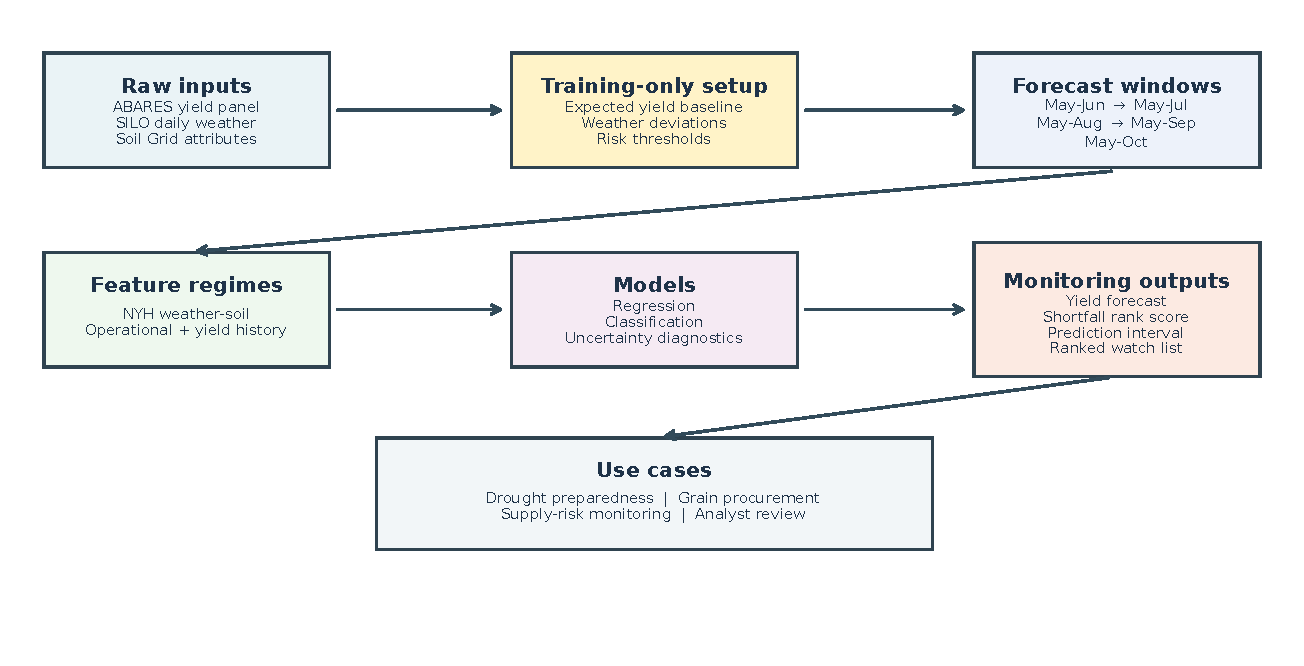
\includegraphics[width=\textwidth]{figures/fig02_stage_aware_workflow.pdf}
\caption{Leakage-safe stage-aware monitoring workflow. Raw yield, weather, and soil inputs are converted into training-only baselines and cutoff-specific feature windows. Separate no-yield-history and operational regimes distinguish within-season environmental signal from historical crop-region yield memory. Outputs are designed for state-level ranked watch lists rather than automatic farm-level decisions.}
\label{fig:workflow}
\end{figure}
\FloatBarrier

\subsection{Prediction Targets}

The regression target is yield in tonnes per hectare, denoted $y_{r,c,t}$. We also define an expected-yield baseline from training years and the shortfall
\[
  s_{r,c,t} = \hat{y}^{\mathrm{exp}}_{r,c,t} - y_{r,c,t}.
\]
The expected-yield baseline is fitted using training years only. In the main specification, expected yield is estimated from a crop-region linear trend in calendar year; crop-level linear trends are used when a crop-region series is too short, and the overall training mean is the final tier in this training-only hierarchy. This baseline excludes current-season weather, production, area, lagged yield, and all validation/test outcomes. Validation and test shortfalls are then computed by applying the fixed training-period baseline to later years. The binary low-yield-risk label is one when shortfall exceeds the crop-specific 80th percentile of the training distribution. We use this threshold as a broad watch-list definition rather than as a severe crop-failure definition. This target follows the general idea that yield anomalies or shortfalls require a reference trend before climate impacts can be assessed \citep{meng2024detrending}, but here the shortfall is used for early-warning classification rather than post-hoc causal attribution. The classification target is used for secondary risk-alert analyses; the main quantitative results remain regression and ablation metrics.

\subsection{Feature Construction and Model Regimes}

For each forecast window $w$, daily weather is aggregated only from May through the cutoff month of $w$. The design intentionally mimics an operational update: May-Jun uses only two months of weather, while May-Oct uses the longest pre-harvest window. No weather feature uses data after the cutoff month. This makes the lead-time comparison interpretable as a sequence of information sets rather than a single full-season model.

The weather feature groups are rainfall accumulation and dry spells, heat and cold exposure, radiation and evaporative demand, and compound hot-dry stress. These choices are motivated by stage-aware and extreme-weather yield studies \citep{schierhorn2021developmentalStages,heino2023hotDryExtremes,heilemann2024lassoExtremes}. We additionally construct weather-deviation features by subtracting train-period region-window baselines. This produces rainfall, temperature, dry-spell, heat-day, evapotranspiration, and radiation deviations that are comparable across regions and forecast windows. The weather-deviation baselines are computed using training years only, so they do not leak test-period information. Feature groups and ablation regimes are listed in the supplementary material.

We report two primary feature regimes. The no-yield-history weather-soil regime uses stage weather features, train-derived weather-deviation features, soil background features, crop identity, region identity, and year. It excludes lagged yield, rolling yield, production, and area; it is not free of crop, state-level region, or time structure. The operational with yield history regime adds past-yield features from prior years for the same crop-region series. This makes it useful for deployment in known crop-region histories, but it is not interpreted as pure weather evidence.

The model suite combines regularized linear baselines with gradient-boosted tabular models. Ridge and ElasticNet provide stable small-data baselines, while LightGBM and CatBoost provide nonlinear tabular comparators \citep{ke2017lightgbm,prokhorenkova2018catboost}. The expanded internal baseline suite also includes Random Forest, SVR-RBF, XGBoost, HistGradientBoosting, GAM, and a daily-weather GRU sequence comparator; implementation details are reported in the supplementary material. To keep the evaluation auditable, performance tables are paired with feature-set ablation, lead-time comparison, or group permutation importance rather than relying on a black-box score alone. This is consistent with the broader argument that high-stakes decision support should prefer transparent or at least carefully audited modeling workflows \citep{rudin2022blackboxBrief}.

Classification models use validation-tuned thresholds for low-yield-risk decisions. Instead of fixing a probability threshold at 0.5, we choose thresholds on validation years for F1, recall constraints, or precision constraints, then report test metrics once. Probabilistic interval diagnostics use quantile-style predictions and conformal calibration ideas as supplementary checks \citep{romano2019cqr,angelopoulos2023conformal}. These outputs are not framed as definitive event decisions; they are screening layers for state-level monitoring.

\subsection{Experimental Setup}

The main split trains on 1989--2012, tunes on 2013--2016, and tests on 2017--2021. The test period is not used for scalers, feature thresholds, residual calibration, conformal residuals, expected-yield baselines, weather-deviation baselines, or low-yield-risk thresholds. This temporal split reflects the intended forecasting direction: models learn from earlier seasons and are evaluated on later seasons.

Regression metrics are MAE, RMSE, and \Rsqdot{} Classification metrics are precision, recall, F1, ROC-AUC, PR-AUC, and Brier score. For probabilistic diagnostics, we summarize interval coverage and width. The conformal intervals target nominal 80\% marginal coverage using validation-period calibration residuals only; test coverage is reported without retuning. When test coverage differs from the nominal level, we interpret the gap as calibration difficulty under temporal shift and small validation samples; we do not tune intervals using test outcomes. The primary model-selection comparisons are always made within the same forecast window and split.

Robustness checks include rolling-origin folds, leave-one-crop-out validation, and leave-one-region-out validation. Rolling-origin validation tests sensitivity to a single time split. Leave-one-crop-out and leave-one-region-out are intentionally difficult transfer tests. We do not treat them as the main deployment setting, because the intended use case is monitoring crop-region combinations with historical observations. Instead, they identify where the framework is not yet robust enough for unseen-crop or unseen-state generalization.

\section{Results}

\subsection{Lead-Time Skill}

Lead-time results show that accuracy generally improves as later-season information becomes available, and that the operational setting outperforms the no-yield-history setting across all forecast windows. By May-Oct, the best operational model reaches RMSE 0.660 t/ha and \Rsq{} 0.728, compared with RMSE 0.821 t/ha and \Rsq{} 0.579 for the best no-yield-history model.

The May-Jun operational result is already informative, with RMSE 0.719 t/ha and \Rsq{} 0.677, but its interpretation is deliberately bounded. It is not early-season weather-only skill; it combines early weather with crop-region memory. The no-yield-history trajectory is weaker and not strictly monotonic, which is plausible in a small state-level panel where later windows add useful weather information alongside correlated features and noise. Detailed lead-time rows are reported in the supplementary material; the lead-time curve should be interpreted as a monitoring trajectory, not as a guarantee that every additional month improves every model.

\begin{figure}[H]
\centering
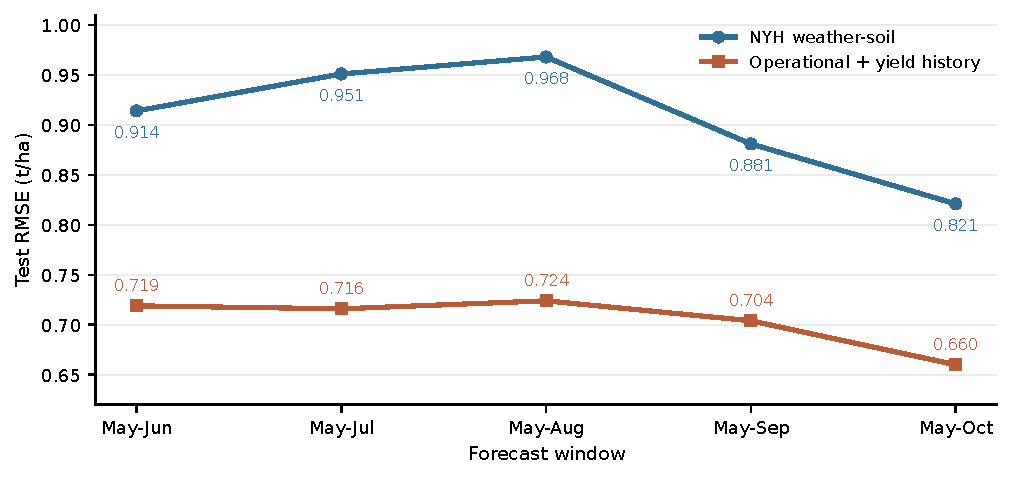
\includegraphics[width=0.82\textwidth]{figures/fig03_lead_time_rmse.pdf}
\caption{Lead-time RMSE comparison between the no-yield-history weather-soil regime and the operational regime with yield history. Lower is better. The curve frames forecasting as a monitoring trajectory rather than a single end-of-season prediction.}
\label{fig:lead-time-rmse}
\end{figure}
\FloatBarrier

\subsection{Comparison with Strong Internal Baselines}

External crop-yield results are difficult to compare directly because reported accuracy depends on crop type, geography, spatial resolution, input modality, target definition, lead time, and evaluation protocol. We therefore compare strong internal baselines and SOTA-style model families within the same leakage-safe evaluation protocol. The comparison includes historical yield baselines, regularized linear models, kernel methods, tree ensembles, gradient-boosted tabular models, interpretable additive models, and a daily-weather GRU sequence comparator, all evaluated on the same Australian state-level panel and chronological split.

\begin{figure}[H]
\centering
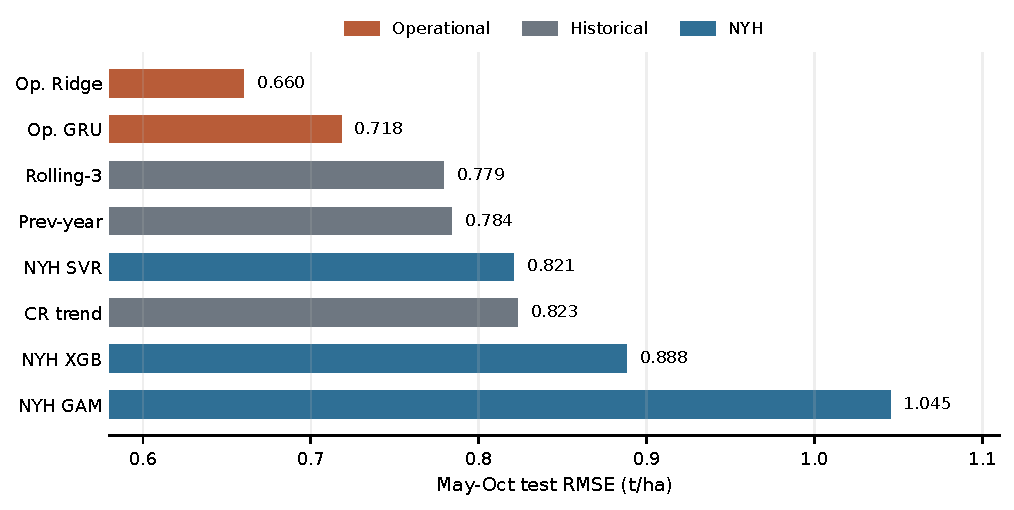
\includegraphics[width=0.82\textwidth]{figures/fig04_baseline_rmse_comparison.pdf}
\caption{May-Oct RMSE comparison across representative strong internal baselines and SOTA-style model families under the same leakage-safe split. Lower is better. Full baseline metrics are reported in the supplementary material.}
\label{fig:baseline-rmse}
\end{figure}
\FloatBarrier

The controlled comparison shows that model class alone does not explain the best performance. Strong boosted and sequence models are competitive, but the best May-Oct result comes from the operational regime with yield-history features. This supports the central interpretation: historical crop-region memory is a major source of operational skill, while weather and soil provide measurable but secondary early-warning information. The no-yield-history models remain useful as an information-isolation benchmark rather than as the strongest deployment model.

\subsection{Low-Yield-Risk Classification}

Risk classification is useful only if it is framed as triage rather than automation. With thresholds chosen on validation years only, the best May-Oct classifier is LogisticRegression with threshold 0.27, precision 0.469, recall 0.556, F1 0.508, ROC-AUC 0.797, PR-AUC 0.390, and Brier score 0.135 on the test period. The May-Oct test prevalence is 18.1\%, so the PR-AUC is above the random-ranking baseline but not high enough for automatic alerts. The tuned threshold improves recall relative to a naive 0.5 cutoff, which is appropriate when missing a shortfall is costly, but modest precision means the output should be a ranked analyst watch list rather than a deterministic event call.

Table~\ref{tab:watch-list-main} shows the intended operational format: a short ranked list for analyst review, not calibrated probabilities or automatic decisions. The warning levels are derived from held-out rank scores only to make the display less probability-like; full threshold sensitivity, confusion-matrix, and ranked watch-list details are reported in the supplementary material.

\begin{table}[H]
\centering
\caption{Example held-out ranked watch list for analyst review. The warning output is designed to prioritize state-crop-year combinations for monitoring rather than to make automatic event decisions.}
\label{tab:watch-list-main}
\begin{tabular}{@{}rlllcc@{}}
\toprule
Rank & Region & Crop & Year & Warning level & Observed risk \\
\midrule
1 & VIC & Oats & 2018 & High & Yes \\
2 & NSW & Lupins & 2018 & High & Yes \\
3 & VIC & Lupins & 2018 & High & No \\
4 & VIC & Canola & 2018 & High & No \\
5 & NSW & Wheat & 2018 & Medium & Yes \\
\bottomrule
\end{tabular}

\end{table}
The false positives in the top ranks illustrate why the output is used for triage and analyst review rather than automatic decision-making.
\FloatBarrier

\subsection{Stress Validation}

Stress validation narrows the supported deployment setting. Rolling-origin validation remains comparatively strong, suggesting that the main temporal holdout result is not driven only by one favorable train-test boundary. Performance declines under harder transfer settings, especially when the model is evaluated on unseen regions. This pattern supports the intended use case of monitoring known crop-region histories while warning against extrapolating the system to unseen state-level regions without recalibration.

Leave-one-crop-out is substantially harder for the no-yield-history model, which is expected because crop identity changes the yield scale and sensitivity to weather. Leave-one-region-out remains the hardest setting, supporting the limitation that unseen-state transfer requires recalibration. Detailed stress-validation rows and a heatmap view are included in the supplementary material.

\begin{figure}[H]
\centering
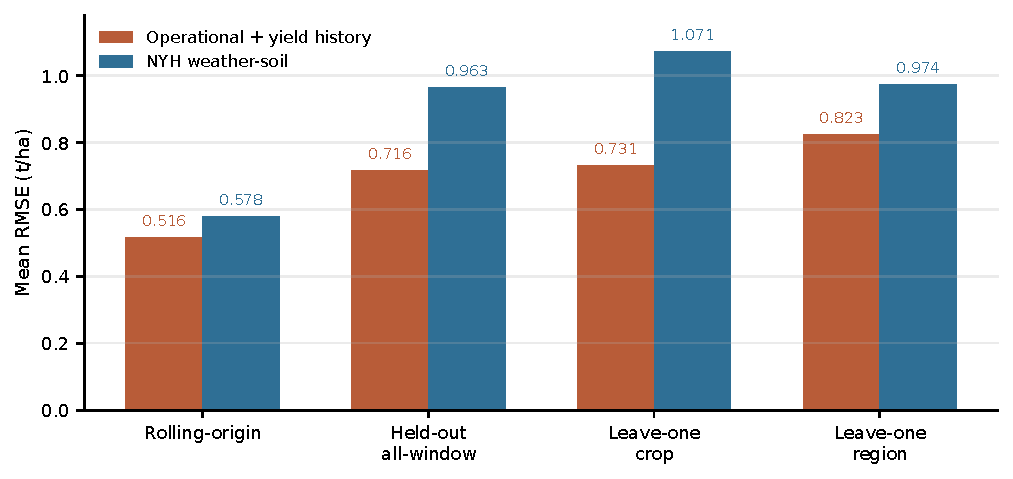
\includegraphics[width=0.82\textwidth]{figures/fig05_stress_validation_rmse.pdf}
\caption{Stress-validation RMSE comparison across validation protocols and feature regimes. Lower is better. Leave-one-region-out remains the hardest setting, supporting the limitation that unseen-state transfer requires recalibration.}
\label{fig:stress-rmse}
\end{figure}
\FloatBarrier

\subsection{Feature Group Importance}

Group permutation importance reinforces the ablation interpretation. Lag-yield features dominate the operational model, especially in early windows where less current-season weather has accumulated. In the no-yield-history setting, soil background, categorical/time structure, and heat/cold features are among the most important groups, while rainfall and dry-spell features contribute less consistently. These patterns support monitoring and vulnerability conditioning rather than causal attribution: the model identifies useful statistical signals, but the design is not an intervention study. The full feature-importance figure is reported in the supplementary material.

\section{Discussion}

The results highlight a practical distinction: a warning based on current-season weather and soil should be interpreted differently from one that also uses historical yield memory. The no-yield-history weather-soil model indicates that stage-aware weather and soil variables contain measurable but secondary early-warning information, whereas the operational model is more accurate because it also uses historical yield memory. In practice, the output is best used as a ranked review list: agencies, grain handlers, procurement planners, and drought-preparedness teams can use early windows for triage and later windows for pre-harvest supply-risk assessment. The system is not intended to replace expert judgment or make automatic decisions.

The supported use case is bounded in several ways. The study is state-level, not farm-level, and the soil variables are static regional covariates rather than causal interventions. The common May-Oct calendar does not fully represent crop-specific phenology, the panel is small for modern machine learning, and leave-one-region-out validation shows weak transfer to unseen states. Residual checks also support a cautious interpretation: after crop-region trends are removed, weather-soil residual models do not outperform the direct no-yield-history setup, reinforcing that much state-level predictability is tied to persistent regional structure. The outputs should therefore not be used for field-scale management, insurance payout decisions, causal attribution, or deployment in unseen regions without recalibration.

Future work should prioritize factors that would make deployment more reliable, including finer spatial labels, crop-area-weighted weather exposure, remote-sensing features, crop-specific phenological windows, stronger transfer learning for unseen regions, and larger calibration sets.

\section{Conclusion}

Framing crop-yield forecasting as stage-aware early warning shifts the task from a single final prediction to a sequence of seasonal risk updates. In this Australian winter-crop evaluation, the best operational May-Oct model reached RMSE 0.660 t/ha and \Rsq{} 0.728, while the best no-yield-history weather-soil May-Oct internal-suite model reached RMSE 0.821 t/ha and \Rsq{} 0.579. The gap between these regimes shows that weather and soil provide measurable but secondary early-warning information, while historical yield memory is central to the strongest operational forecasts. These results support ranked state-level yield-risk review for known crop-region histories, while limiting claims to monitoring support rather than farm-level decisions, causal attribution, automatic decisions, or unseen-region transfer.

\noindent\textbf{Code availability.}
Code and reproducibility scripts are available at:\par
\url{https://anonymous.4open.science/r/acml2026-crop-warning-review-E32F}

\begingroup
\small
\setlength{\bibsep}{0pt}
\bibliography{acml26}
\endgroup

\end{document}
